%! TEX root = ../../master.tex
\lecture[General matchings via $\LP$. Prerequisites for blossom algorithm.]{Do 02 June 2022}{General matchings}

\subsection{Combinatorial algorithms for $\IP$}
\begin{definition}
    Given a graph $G=(N,E)$ and matching $M$.
    \begin{enumerate}
        \item A path is \vocab{alternating} w.r.t. $M$
              if its edges alternate between $M$ and $E-M$.
        \item A node is \vocab{exposed} if no edge in $M$ hits the node.
        \item A path is \vocab{augmenting} if it is alternating and both endpoints are exposed.
    \end{enumerate}
\end{definition}
\begin{theorem}
    A matching $M$ is not maximum iff there exist an augmenting path w.r.t. $M$.
\end{theorem}
\begin{proof}
    The reverse is clear. Thus, consider a non-maximum matching $M$. Then there
    is a matching $M'$ with $|M'|=|M|+1$. Let $D=M \Delta M'$, thus
    \begin{align*}
        |D|=|M|+|M'|-2|M \cap M'| \ \text{is odd}
    \end{align*}
    $D$ is possibly composed into \todo{some graphics alternating}.

    This implies thiat there is a alternating path of odd length.
    Note $|M'-M|>|M-M'|$, so there is an $M$-augmenting path.
\end{proof}
We can use this theorem to possibly create an algorithm!
\begin{recall}
    The cardinality of a matching is at most the cardinality of a node cover.
    For the special case of bipartite graphs, König's theorem state that they are even equal.
\end{recall}
\begin{theorem}[\vocab{Tutte-Berge}]
    For $G=(N,E)$,
    \begin{align*}
        \max_{\text{matching } M}|M|= \min_{X \subseteq V} \frac{1}{2}(|V|-\oc(X)+|X|)
    \end{align*}
    where oc$(X)$ is the number of  odd components in $G(V-X)$.
\end{theorem}
\begin{proof}[Proof of $\leq$]
    Let $X \subseteq V$ be such that $G(V-X)$ has $k$ odd components $H_i$.
    Let $M$ be a matching. For each $H_i$, either there exist a $M$-exposed node,
    or there exist an edge in $M$ from $H_i$ to $X$.

    The number of such edges is at most $|X|$, therefore there must be at least $k - |X|$ exposed nodes.
    Because these nodes are by definition not in the matching, there remain only at most
    the right side of our equation many matched edges.
\end{proof}
\begin{proof}[Proof of $\geq$]
    See tutorial.
\end{proof}
\begin{definition}
    For an odd cycle $C$ in $G$, we define $G' \coloneqq G \times C$ to be the following graph:
    \\
    \begin{minipage}{\textwidth}
        \centering
        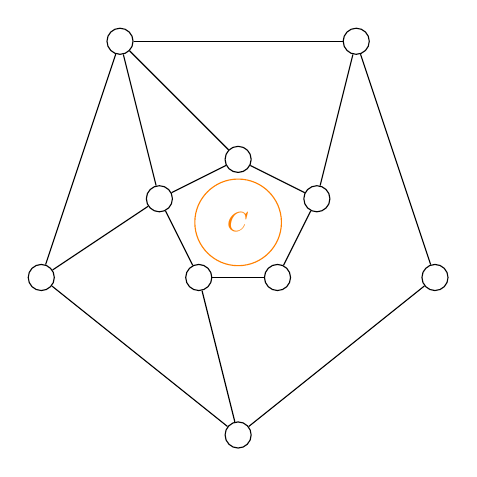
\begin{tikzpicture}
            \begin{scope}[
                    every node/.style={circle, draw},
                    every edge/.style={draw, semithick}
                ]

                \node (o1) at (2.5,0) {};
                \node (o2) at (5,2) {};
                \node (o3) at (4,5) {};
                \node (o4) at (1,5) {};
                \node (o5) at (0,2) {};

                \node (i1) at (2,2) {};
                \node (i2) at (3,2) {};
                \node (i3) at (3.5,3) {};
                \node (i4) at (2.5,3.5) {};
                \node (i5) at (1.5,3) {};
            \end{scope}

            % \draw[red, very thick] (l1) -- (r2);
            % \draw[red, very thick] (l2) -- (r3);
            \draw (o1) edge (o2);
            \draw (o2) edge (o3);
            \draw (o3) edge (o4);
            \draw (o4) edge (o5);
            \draw (o5) edge (o1);
            \draw[orange] (2.5,2.7) circle (0.55);
            \node[orange] (C) at (2.5,2.7) {$C$};

            \draw (i1) edge (i2);
            \draw (i2) edge (i3);
            \draw (i3) edge (i4);
            \draw (i4) edge (i5);
            \draw (i5) edge (i1);

            \draw (o1) edge (i1);
            \draw (o3) edge (i3);
            \draw (o4) edge (i4);
            \draw (o4) edge (i5);
            \draw (o5) edge (i5);
            % \end{scope}
        \end{tikzpicture}
        % \captionof{figure}{A graph with the spanning tree in black and arc subset $S$ in orange}
    \end{minipage}
    \vspace{5pt}
    \\
\end{definition}
Given $G$ and $C$, let $M'$ be a matching in shrinked $G'$, and let $M$ be an extended
matching in $G$. Then, the number of $M$-exposed nodes in $G$ is the same as for $M'$ in $G'$.
\begin{warning}
    By this procedure, it is \emph{not} true that $M$ is maximum iff $M'$ is maximum.
\end{warning}

Given $G,M,$ and odd cycle $C$ such that
\begin{align*}
    |M \cap C| = \frac{|C|-1}{2}.
\end{align*}
Let $c \in C$ be the one not covered within $C$. Suppose that for any $M$-exposed
node $r$, all alternating $r-c$-paths are disjoint from $V(C)-c$.
\begin{theorem}
    By this procedure, $M$ is maximum in $G$ iff $M'$ is maximum in $G'$.
\end{theorem}
\begin{proof}
    First, suppose $M$ is maximum, but $M'$ is not. Then $|M'|=|M|-k$ with
    \begin{align*}
        k \coloneqq |M \cap C| = \frac{|C|-1}{2}.
    \end{align*}
    If there exists a matching $N'$ in $G'$ with $|N'|>|M'|$, then there exists a matching $N$ in $G$
    with
    \begin{align*}
        |N| = |N'|+k > |M|
    \end{align*}
    Contradiction!

    For the other direction, suppose $M'$ is maximum, but $M$ is not.
    Then there exists an augmenting path $P$ in $G$.
    Let $v$ be an endnode of $P$ that is not in $V(C)$, and consider two cases:
    \begin{itemize}
        \item $P \cap C = \emptyset$: Let $w$ be the other endnode.
        \item $P \cap C \neq \emptyset$: Let $w$ be the first node on $P$ in $V(C)$.
              As a consequence, the $v-w$-path is $M'$-augmenting - contradiction!
    \end{itemize}
    \todo{graphic}
\end{proof}
\begin{algorithm}[H] \label{algo:alt_tree}
    \SetAlgoLined
    Graph $G$, matching $M$, exposed node $r$\\
    $A \leftarrow \emptyset$\\
    $B \leftarrow \{r\}$\\
    \While{for any $w \in V$: $(u,v)\in E, u \in B, v \in A \cup B, (v,w)\in M$}{
        $A \leftarrow A + v$\\
        $B \leftarrow B + w$\\
    }
    %  reindeer $\leftarrow$ 0\tcp*{current position of reindeer} 
    \caption{Alternating tree-algorithm}
\end{algorithm} \noindent
\todo{graph}
Notice that $A$ ($B$) contains all nodes that are endnodes of an odd (even)-length $M$-alternating path on $T$.
\begin{definition}
    The tree we get by \autoref{algo:alt_tree} is called $M$-\vocab{alternating tree}.
\end{definition}
\begin{observe} Using this algorithm we see
    \begin{itemize}
        \item every note other than $r$ is covered by an edge in $M \cap E(T)$,
        \item every path from $r$ to any $v \in V(T)$ in $T$ is alternating,
        \item $|B|=|A|+1$
    \end{itemize}
\end{observe}
Any $(u,v) \in E$ with $u,v \in B$ forms an odd cycle $C$, shrinking it to node $c$
(and adding $c$ to $B$) does not affect our structure.

If $m$-alternating trees from two roots $r_1, r_2$ share an $(u,v) \in E$ with
$u \in B_1, v \in B_2$, then there exists an $M$-augmenting path from $r_1$ to $r_2$.